\chapter{Mở đầu đại số Boolean}

Boolean (hay luận lý) chỉ giá trị đúng hoặc sai của mệnh đề nào đó. 
Theo cách hiểu cơ bản, boolean gồm 2 giá trị 0 hoặc 1 (sai hoặc đúng).

\section{Hàm Boolean}

Hàm boolean $f$ đối với các biến $x_1, x_2, \ldots, x_n$ là hàm số 
nhận giá trị trong $\FF_2^n$ và trả về giá trị thuộc $\FF_2$.

Nghĩa là $f: \FF_2^n \mapsto \FF$

Ta ký hiệu hàm boolean $n$ biến là $f(x_1, x_2, \ldots, x_n)$.

Do $x_i \in \FF_2$ nên ta có $2^n$ vector (bộ số)
$(x_1, x_2, \ldots, x_n)$. Giá trị của hàm $f$ lại nằm
trong tập $\{0, 1\}$ nên ứng với mỗi vector có thể có 2 giá 
trị của hàm boolean, và ta có $2^n$ vector nên số lượng hàm
boolean có thể có là $2^{2^n}$.

Một số toán tử boolean hay dùng: đối, AND, OR, XOR, NAND, NOR, 
kéo theo, tương đương.

Để biểu diễn hàm boolean chúng ta dùng bảng chân trị. Bảng chân
trị tương ứng với các toán tử boolean trên là:

\begin{table}[ht]
    \centering
    \begin{tabular}{|c|c|c|c|c|c|c|}
        \hline
        & & AND & OR & XOR & NAND & NOR \\
        $x_1$ & $x_2$ & $x_1 \cdot x_2$ & $x_1 \vee x_2$ &
            $x_1 \oplus x_2$ & $x_1 \vert x_2$ &
            $x_1 \downarrow x_2$ \\
        \hline
        0 & 0 & 0 & 0 & 0 & 1 & 1 \\
        \hline
        0 & 1 & 0 & 1 & 1 & 1 & 0 \\
        \hline
        1 & 0 & 0 & 1 & 1 & 1 & 0 \\
        \hline
        1 & 1 & 1 & 1 & 0 & 0 & 0 \\
        \hline
    \end{tabular}
    \caption{Các toán tử AND, OR, XOR, NAND, NOR}
\end{table}

Toán tử đối làm đổi giá trị của hàm bool (0 thành 1 và 1 thành 0).
Ký hiệu $\overline{x}$.

\begin{table}[ht]
    \begin{subtable}[t]{0.25\textwidth}
        \centering
        \begin{tabular}{|c|c|}
            \hline
            $x$ & $\overline{x}$ \\
            \hline
            0 & 1 \\
            \hline
            1 & 0 \\
            \hline
        \end{tabular}
        \caption{Toán tử đối}
    \end{subtable}
    \hspace{\fill}
    \begin{subtable}[t]{0.55\textwidth}
        \centering
        \begin{tabular}{|c|c|c|c|}
            \hline
            $x_1$ & $x_2$ & $x_1 \rightarrow x_2$ & $x_1 \sim x_2$ \\
            \hline
            0 & 0 & 1 & 1 \\
            \hline
            0 & 1 & 1 & 0 \\
            \hline
            1 & 0 & 0 & 0 \\
            \hline
            1 & 1 & 1 & 1 \\
            \hline
        \end{tabular}
        \caption{Toán tử kéo theo và tương đương}
    \end{subtable}
    \caption{Các toán tử đối, kéo theo, tương đương}
\end{table}

Toán tử tương đương còn chỉ sự tương đương của hai mệnh đề logic.
Khi hai biểu thức logic có cùng bảng chân trị thì hai mệnh đề đó
tương đương nhau. Do đó ta có thể viết một số kết quả như sau (từ
các bảng chân trị cơ bản trên):

\begin{itemize}
    \item $x_1 \vert x_2 \sim \overline{x_1 \cdot x_2}$. Ở đây
        ta đổi dấu từng giá trị hàm boolean $x_1 \cdot x_2$
    \item $x_1 \downarrow x_2 \sim \overline{x_1 \vee x_2}$. 
        Tương tự ta đổi dấu từng giá trị hàm boolean $x_1 \vee x_2$
\end{itemize}

\section{Đa thức Zhegalkin}

\begin{definition}[Đa thức Zhegalkin]
    Với hàm boolean $n$ biến $f(x_1, x_2, \ldots, x_n)$, đa thức Zhegalkin tương ứng với hàm bool đó là cách biểu diễn
    đa thức đó dưới dạng tổng các tích như sau
    \begin{equation}
        f(x_1, x_2, \ldots, x_n) = a_0 \oplus a_1 x_1 
        \oplus a_2 x_2 \oplus a_3 x_1 x_2 \oplus \ldots 
        \oplus a_k x_1 x_2 \ldots x_n
    \end{equation}
    với $a_i \in \{0, 1\}$. Ta thấy rằng có $n$ biến, do đó có 
    $2^n$ hệ số $a_i$ ($k = 2^n$).
\end{definition}

Khi đó ta nói hàm boolean $f$ được biểu diễn ở \textit{dạng
chuẩn tắc đại số} (algebraic normal form).

\begin{example}
    Cho hàm bool $f(x, y) = x \vee y$. Ta có bảng chân trị sau
    \begin{table}[ht]
        \centering
        \begin{tabular}{|c|c|c|}
            \hline
            $x$ & $y$ & $f(x, y)$ \\ \hline
            0 & 0 & 0 \\ \hline
            0 & 1 & 1 \\ \hline
            1 & 0 & 1 \\ \hline
            1 & 1 & 1 \\ \hline
        \end{tabular}
    \end{table}

    Bảng chân trị này tương đương với đa thức Zhegalkin
    \[f(x, y) = x \oplus y \oplus xy\]
\end{example}

\begin{definition}[Bậc của đa thức Zhegalkin]
    Tương tự như bậc của một đa thức đại số thông thường,
    bậc của đa thức Zhegalkin là bậc của hạng tử chứa nhiều
    đơn thức $x_i$ nhất. Ký hiệu là $deg(f)$.
\end{definition}

\begin{example}
    Xét hàm boolean $f(x, y, z) = 1 \oplus x \oplus yz \oplus xyz$.
    Khi đó $deg(f) = 3$ vì hạng tử chứa nhiều đơn thức nhất là $xyz$
    có 3 đơn thức.

    Xét hàm boolean $f(x, y, z) = 1 \oplus z \oplus zy \oplus xy$. 
    Khi đó $deg(f) = 2$ vì hạng tử chứa nhiều đơn thức nhất là
    $zy$ (cũng có thể xét $xy$).
\end{example}

\section{Cách tìm đa thức Zhegalkin từ bảng chân trị}

Ta có nhiều phương pháp để tìm đa thức Zhegalkin của một hàm 
boolean từ bảng chân trị. 

\subsection{Phương pháp tam giác}

Ở hàng đầu ta viết các phần
tử bảng chân trị từ trái sang phải. Với $n$ biến sẽ có $2^n$ ô.
Hàng thứ hai có $2^n-1$ ô. Phần tử dưới sẽ bằng XOR của 2 phần tử 
ngay trên nó (tạo thành tam giác). Tiếp tục như vậy tới khi
ta có hàng cuối chỉ có 1 ô.

\begin{figure}[ht]
    \centering
    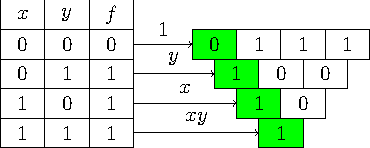
\includegraphics{../pics/boolean/zhegalkin1.pdf}
    \caption{Phương pháp tam giác}
\end{figure}

Khi đó, tương ứng với các biến, nếu biến đó là 1 thì hạng tử chứa
biến đó, 0 thì không ghi. Ở ví dụ trên, nếu $(x, y) = (0, 0)$ 
thì không có gì (phần tử 1), $(x, y) = (0, 1)$ tương ứng với hạng 
tử $y$ trong đa thức Zhegalkin, $(x, y) = (1, 0)$ tương ứng hạng
tử $x$. Cuối cùng $(x, y) = (1, 1)$ tương ứng hạng tử $xy$.

Hệ số trước mỗi hạng tử là phần tử đầu tiên bên trái theo bảng
kim tự tháp. Như vậy đa thức Zhegalkin là:
\begin{equation*}
    f(x, y) = 0 \cdot 1 \oplus 1 \cdot y \oplus 1 \cdot x \oplus 
        1 \cdot xy = x \oplus y \oplus xy
\end{equation*}

Đa thức Zhegalkin đóng vai trò quan trọng trong nhiều lĩnh vực,
bao gồm cả toán học, vật lý, khoa học máy tính, vì AND và XOR
là hai toán tử đại số cơ bản, do đó biểu diễn đa thức Zhegalkin
được gọi là dạng chuẩn tắc đại số như ở trên đề cập.

Một ví dụ khác của đa thức Zhegalkin với hàm 3 biến $x$, $y$ và $z$
như hình sau:

\begin{figure}[ht]
    \centering
    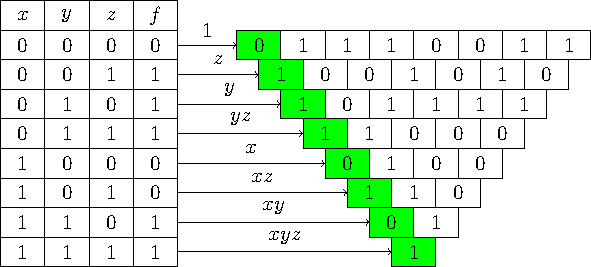
\includegraphics{../pics/boolean/zhegalkin2.pdf}
\end{figure}

Như vậy ứng với hàm boolean $f$ thì đa thức Zhegalkin là:
\begin{equation*}
    f(x, y, z) = z \oplus yz \oplus x \oplus xz \oplus xyz
\end{equation*}

\subsection{Phương pháp \foreignlanguage{german}{Möbius}}

Phương pháp này cho phép chúng ta tính hệ số đa thức Zhegalkin
như phương pháp tam giác nhưng nhanh hơn và đỡ sai sót hơn.

Đầu tiên chúng ta chia đôi bảng chân trị thành hai nửa trái phải.
Nửa trái giữa nguyên, mỗi phần tử ở nửa phải được XOR (cộng modulo 2)
với phần tử tương ứng ở nửa trái.

Giả sử với hàm $f(x, y) = (0, 1, 1, 1)$ như trên. Bước 1, ta giữ
nguyên 2 phần tử đầu 0 và 1. Phần tử thứ ba (mới) bằng
phần tử thứ ba (cũ) XOR với phần tử đầu ($0 \oplus 1 = 1$).
Phần tử thứ tư (mới) bằng phần tử thứ tư (cũ) XOR với phần tử
thứ hai ($1 \oplus 1 = 0$).

Tiếp theo, chúng ta xử lý như trên cho 2 phần tử bên nửa trái 
(2 phần tử bên nửa phải xử lý tương tự).

\begin{figure}[ht]
    \begin{subfigure}{0.45\textwidth}
        \centering
        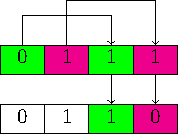
\includegraphics{../pics/boolean/zhegalkin3.pdf}
        \caption{Bước 1}
    \end{subfigure}
    \hfill
    \begin{subfigure}{0.45\textwidth}
        \centering
        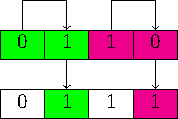
\includegraphics{../pics/boolean/zhegalkin4.pdf}
        \caption{Bước 2}
    \end{subfigure}
\end{figure}

Như vậy ta có kết quả là $(0, 1, 1, 1)$, tương ứng với các
hạng tử $1$, $y$, $x$, $xy$ (như trên). Vậy đa thức Zhegalkin
là $f(x, y) = x \oplus y \oplus xy$.

\section{Các hàm boolean và tính chất}

\begin{definition}[Hàm boolean Affine]
    Xét hàm boolean $n$ biến $f(x_1, x_2, \ldots, x_n)$.
    Khi đó $f$ được gọi là
    \textit{hàm boolean Affine} nếu nó có dạng
    \begin{equation}
        f(x_1, x_2, \ldots, x_n) = a_0 \oplus a_1 x_1 \oplus 
        a_2 x_2 \oplus \ldots \oplus a_n x_n
    \end{equation}
    Khi $a_0 = 0$ thì ta gọi là \textit{hàm boolean tuyến tính}
    (linear).
\end{definition}

Ta thấy rằng chỉ có các hạng tử dạng $a_i x_i$ xuất hiện trong
biểu diễn đa thức Zhegalkin tương ứng của hàm boolean đó. Hay 
nói cách khác hàm boolean là Affine khi $deg(f) = 1$.

\begin{example}
    Hàm boolean $f(x, y) = x \oplus y$ là hàm boolean Affine và
    cũng tuyến tính. Hàm boolean $f(x, y) = x \oplus xy$ không là 
    hàm boolean Affine.
\end{example}

Tiếp theo ta sẽ xét sự so sánh của hai vector và 
hàm boolean đơn điệu.

\begin{definition}[Vector so sánh được]
    Xét hai bộ $n$ số (vector) $\bar{a} = (a_1, a_2, \ldots, a_n)$ 
    và $\bar{b} = (b_1, b_2, \ldots, b_n)$ ($a_i, b_i \in \{0, 1\}$). 
    Ta nói $\bar{a}$ so 
    sánh được nhỏ hơn $\bar{b}$ nếu với mọi $i = 1, 2, \ldots, n$
    ta có $a_i \leq b_i$. Ký hiệu $\bar{a} \prec \bar{b}$.
\end{definition}

\begin{example}
    Ta có $(1, 0, 0) \prec (1, 0, 1)$, còn $(1, 0, 0)$ và $(0, 1, 0)$
    thì không so sánh được (vị trí thứ 1 và thứ 2).
\end{example}

\begin{definition}[Hàm boolean đơn điệu]
    Hàm boolean $n$ biến $f(x_1, x_2, \ldots, x_n)$ được gọi là
    \textit{hàm boolean đơn điệu} (monotone) nếu với mọi bộ $n$ số
    $(a_1, a_2, \ldots, a_n) \prec (b_1, b_2, \ldots, b_n)$
    thì ta có 
    \begin{equation}
        f(a_1, a_2, \ldots, a_n) \leq f(b_1, b_2, \ldots, b_n)  
    \end{equation}
\end{definition}

\begin{example}
    Xét hàm boolean $f(x, y) = (0, 1, 0, 1)$.

    Ta thấy rằng:
    \begin{itemize}
        \item $(0, 0) \prec (0, 1)$ và $f(0, 0) = 0 \leq 1 = f(0, 1)$
        \item $(0, 0) \prec (1, 0)$ và $f(0, 0) = 0 \leq 0 = f(1, 0)$
        \item $(0, 0) \prec (1, 1)$ và $f(0, 0) = 0 \leq 1 = f(1, 1)$
        \item $(0, 1)$ và $(1, 0)$ không so sánh được nên bỏ qua
        \item $(0, 1) \prec (1, 1)$ và $f(0, 1) = 1 \leq 1 = f(1, 1)$
        \item $(1, 0) \prec (1, 1)$ và $f(1, 0) = 0 \leq 1 = f(1, 1)$
    \end{itemize}

    Vậy đây là hàm đơn điệu.
\end{example}

\section{Trọng số của hàm boolean}

\begin{definition}[Trọng số hàm boolean]
    \textit{Trọng số} (weight) của hàm boolean $n$ biến
    $f(x_1, x_2, \ldots, x_n)$ là số lượng giá trị 1 của
    hàm $f$. Ký hiệu là $w(f)$.
\end{definition}

\begin{example}
    Hàm boolean $f(x, y) = (0, 1, 0, 1)$ có trọng số $w(f) = 2$.
    Hàm boolean $f(x, y, z) = (1, 0, 1, 1, 1, 0, 0, 1)$ có
    trọng số $w(f) = 5$.
\end{example}

Một số tính chất của trọng số:

\begin{enumerate}
    \item $0 \leq w(f) \leq 2^n$
    \item $w(f \oplus 1) = 2^n - w(f)$
    \item Nếu $h$ cũng là một hàm boolean từ $\FF_2^n$ tới 
        $\FF_2$ thì \[w(f \oplus h) = w(f) + w(h) - 2w(fh)\]
    \item Giá trị $w(f)$ nhận giá trị lẻ khi và chỉ khi $deg(f) = n$
\end{enumerate}

\section{Biến đổi Fourier}

Với mỗi vector $a = (a_1, \ldots, a_n) \in \FF_2^n$, ta ký
hiệu $(a, x)$ là hàm sau:
\begin{equation}
    (a, x) = a_1 x_1 + a_2 x_2 + \ldots + a_n x_n
\end{equation}

Mỗi hàm boolean sẽ được biểu diễn dưới dạng duy nhất với

\begin{equation}
    f(x) = 2^{-n} \sum_{a \in \FF_2^n} C_a (-1)^{(a, x)}
\end{equation}

Trong đó
\begin{equation}
    C_a = C_a (f) = \sum_{x \in \FF_2^n} f(x) (-1)^{(a, x)}
\end{equation}

Khi đó, tập hợp $\{C_a (f), a \in \FF_2^n \}$ được gọi là 
\textbf{phổ Fourier} (spectre) Fourier của hàm boolean $f(x)$.

\begin{example}
    Xét hàm boolean $f(x_1, x_2) = (1, 0, 0, 1)$.

    Xét $a = (0, 0)$. Ta có:
    \begin{itemize}
        \item Với $x = (0, 0)$, $f(x) = 1$, $(a, x) =
        0 \cdot 0 + 0 \cdot 0 = 0$.
        \item Với $x = (0, 1)$, $f(x) = 0$, $(a, x) = 
        0 \cdot 0 + 0 \cdot 1 = 0$
        \item Với $x = (1, 0)$, $f(x) = 0$, $(a, x) = 
        0 \cdot 1 + 0 \cdot 0 = 0$
        \item Với $x = (1, 1)$, $f(x) = 1$, $(a, x) = 
        0 \cdot 1 + 0 \cdot 1 = 0$
    \end{itemize}
    Suy ra $C_a = 1 \cdot (-1)^0 + 0 \cdot (-1)^0 + 0 \cdot (-1)^0
        + 1 \cdot (-1)^0 = 2$ khi $a = (0, 0)$.

    Tương tự, ta có các giá trị $C_a$ sau:
    \begin{itemize}
        \item Với $a = (0, 1)$, $C_a = 0$
        \item Với $a = (1, 0)$, $C_a = -1$
        \item Với $a = (1, 1)$, $C_a = 1$
    \end{itemize}
\end{example}

\section{Biến đổi Walsh-Hadamard}

Với mỗi hàm boolean $f(x)$ ta định nghĩa một hàm tương ứng như sau:
\[f^*(x) = (-1)^{f(x)}\]

Ta định nghĩa $(a, x)$ như trên, khi đó hàm $f^*(x)$ sẽ có dạng
\begin{equation}
    f^*(x) = 2^{-n} \sum_{a \in \FF_2^n} z_a (-1)^{(a, x)}
\end{equation}

Trong đó
\begin{equation}
    z_a = z_a (f) = \sum_{x \in \FF_2^n} (-1)^{f(x) + (a, x)}
\end{equation}

Tập hợp $\{z_a(f), a \in \FF_2^n\}$ được gọi là \textbf{phổ
Walsh} (spectre) của hàm $f(x)$. Các giá trị $z_a$ được gọi là hệ số
Walsh.

Các hệ số Walsh liên hệ với nhau bởi công thức

\begin{equation}
    \sum_{a \in \FF_2^n} z_a(f) z_{a+d}(f) = 
    \begin{cases}
    2^{2n}, & d = 0 \\
    0, & d \neq 0
    \end{cases}
\end{equation}

Trường hợp $d = 0$ được gọi là \textit{đẳng thức Parcel}
\begin{equation}
    \sum_{a \in \FF_2^n} z_2^2 = 2^{2n}
\end{equation}